\documentclass[12pt]{article}

\usepackage{amsmath,color,tikz,graphicx,fixltx2e,float}

\setlength{\baselineskip}{16.0pt}    % 16 pt usual spacing between lines

\setlength{\parskip}{3pt plus 2pt}
\setlength{\parindent}{20pt}
\setlength{\oddsidemargin}{0.5cm}
\setlength{\evensidemargin}{0.5cm}
\setlength{\marginparsep}{0.75cm}
\setlength{\marginparwidth}{2.5cm}
\setlength{\marginparpush}{1.0cm}
\setlength{\textwidth}{150mm}
\title{LCR Circuit}
\begin{document}
\maketitle
As we have discussed earlier, \emph{LCR circuit} consists of three elements: \emph{R}esistance, \emph{Inductance} (L), and \emph{C}apacitance, all connected in series and driven by an alternating voltage source. The \emph{LCR} circuit provides a load for the alternating source. Now let us observer what values of impedance are offered by the elements of an LCR circuit by themselves: \\
$$Z_L=j\omega L$$
$L$ is the inductance of the inductor. $\omega$ is the frequency at which it is being driven by an oscillator, and the $j$ in front signifies that the impedance is not real, a matter whose significance will be discussed later on.
$$Z_C=-\frac{j}{\omega C}$$
$C$ is the capacitance of the capacitor.
$$Z_R=R$$
Resistance has no dependence on the frequency of the driver.
Now, when the seperate components are put in series, we know what happens: The impedances add up. So, the impedance of a \emph{LCR} circuit being driven at frequency $\omega$ is given by:
$$
Z=R+j\left(\omega L - \frac{1}{\omega C} \right).
$$
Now, the current through the circuit is same for all elements. So, if the circuit is driven by a supply $v_i=V_0 e^{j \omega t}$, the current is:
$$
i_\omega =\frac{v_i}{Z}=\frac{V_0 e^{j \omega t}}{R+j\left(\omega L - \frac{1}{\omega C} \right)}.
$$
Let us strive a bit to put this in a more convenient form:
$$
\begin{aligned}
i_\omega &=\frac{V_0 e^{j \omega t}}{R+j\left(\omega L - \frac{1}{\omega C} \right)} \\
&=\frac{V_0 e^{j \omega t}}{\left|R+j\left(\omega L - \frac{1}{\omega C} \right)\right|\times e^{j\phi}} \\
&=\frac{V_0 e^{j (\omega t - \phi)}}{\left[R^2+\left(\omega L - \frac{1}{\omega C} \right)^2\right]^{1/2}},
\end{aligned}
$$
with $\phi=\frac{\omega L - \frac{1}{\omega C}}{R}$.
As current and the supply voltage are real quantities, whenever we talk about them all we care about are their real parts. So, the parts of interest are:
$$
\begin{aligned}
v_i &=V_0 \cos \omega t, \\
i &=\frac{V_0 \cos(\omega t - \phi)}{\left[R^2+\left(\omega L - \frac{1}{\omega C} \right)^2\right]^{1/2}}.
\end{aligned}
$$
We observe that the current is not in the same phase as the voltage is. It is lagging (or leading) by a factor $\phi=\frac{\omega L - \frac{1}{\omega C}}{R}$. Note that, the phase shift of the current is entirely due to the presence of the inductor and the capacitor. Had they been absent, there would have been no phase shift. Still, for a given $L$ and $C$, we can find a specific $\omega$ for which $\phi$ is zero. Solving for $\omega$ with this condition, we find that $\omega=1/\sqrt{LC}$, as frequency can never run negative. This special frequency is known as the resonant frequency of the \emph{LCR} circuit, for reasons that will be clarified in a moment. With the current known, we are now able to determine the potential difference across each of the elements. The old knowledge:
$$
V=I \times R.
$$
Only, here we use $Z$ instead of $R$ to obtain the voltages. \\
So, let us calculate $V_R$, $V_L$, $V_C$ by this means:
$$
v_R=Z_R \times i=R\frac{V_0 e^{j (\omega t - \phi)}}{\left[R^2+\left(\omega L - \frac{1}{\omega C} \right)^2\right]^{1/2}},
$$
$$
v_L=Z_L \times i=j\omega L\frac{V_0 e^{j (\omega t - \phi)}}{\left[R^2+\left(\omega L - \frac{1}{\omega C} \right)^2\right]^{1/2}}, \\
$$
$$
v_C=Z_C \times i=-\frac{j}{\omega C}\frac{V_0 e^{j (\omega t - \phi)}}{\left[R^2+\left(\omega L - \frac{1}{\omega C} \right)^2\right]^{1/2}}.
$$
Observe that, all voltages have picked up the phase factor. Since we are interested only in the real part, let us first decouple $e^{j(\omega t -\phi)}$ into $e^{j\omega t}$ and $e^{-j\phi}$, and take the real parts:
So, $v_R$ becomes:
$$
\begin{aligned}
v_R &=\Re \left(R\frac{V_0 e^{j (\omega t - \phi)}}{\left[R^2+\left(\omega L - \frac{1}{\omega C} \right)^2\right]^{1/2}}\right) \\
&=\frac{R\cos{\phi}}{{\left[R^2+\left(\omega L - \frac{1}{\omega C} \right)^2\right]^{1/2}}}\times V_0 \cos{\omega t}.
\end{aligned}
$$
$v_C$ becomes:
$$
\begin{aligned}
v_C &=\Re{\left(-\frac{j}{\omega C}\frac{V_0 e^{j (\omega t - \phi)}}{\left[R^2+\left(\omega L - \frac{1}{\omega C} \right)^2\right]^{1/2}}\right)} \\
&=\frac{\sin{\phi}}{\omega C{\left[R^2+\left(\omega L - \frac{1}{\omega C} \right)^2\right]^{1/2}}} \times V_0 \cos{\omega t}.
\end{aligned}
$$
Similar expression can be derived for $v_L$ also.
Note that, $v_R=V_0\cos{\omega t}$ at the value of $\omega$ where $\phi$ is zero, that is all of the input signal drops across the resistance only, and the inductor and the capacitor plays no role in power dissipation. This is why this condition is termed as resonance, because only at this frequency is $v_R$, and hence the power dissipation in $R$ is maximum. \\
Note that, RMS values of $v_R$, $v_C$ and $v_L$ does not follow simple forms due to the presence of the sine or cosine terms, along with $1/|Z|$, and the sine or cosine terms make the RMS values oscillate with frequency. A few plots are provided depicting this incidence with two different sets of $R$, $L$ and $C$. Note that, only the scale factors present with $V_0 \cos{\omega t}$ are plotted vs the frequency, as these factor are only of interest. \\
We consider the following two sets: \\
\begin{enumerate}
\item $L=68.7$mH, $C=2.33$$\mu$F, $R=1000 \Omega$.
\item $L=68.7$mH, $C=2.33$$\mu$F, $R=100 \Omega$.
\end{enumerate}
The two plots are of set 1 and set 2 respectively:
\begin{figure}[H]
\centering
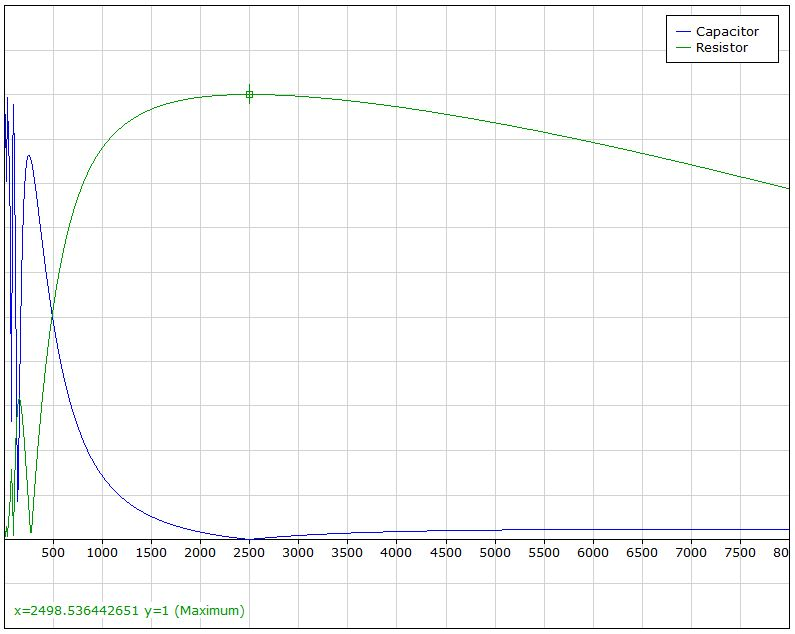
\includegraphics[scale=0.5]{1000}
\end{figure}
\begin{figure}[H]
\centering
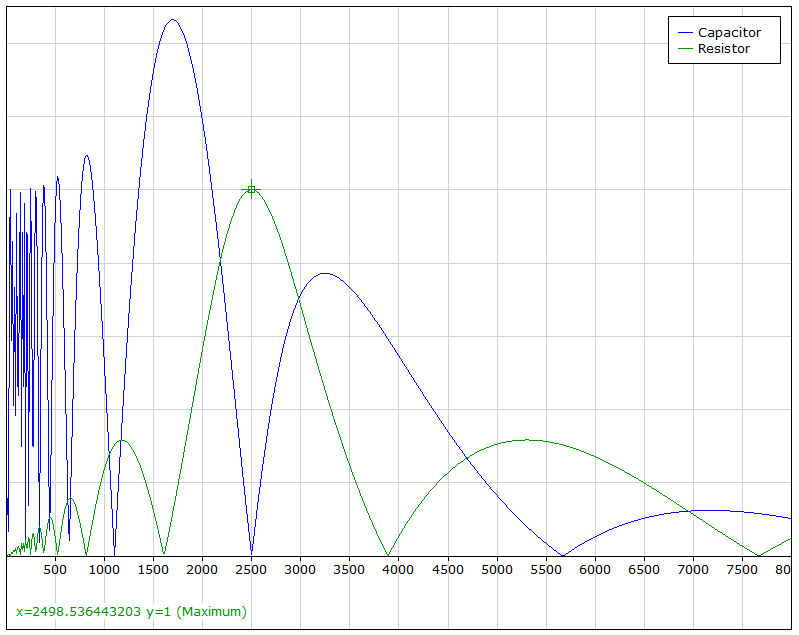
\includegraphics[scale=0.5]{100}
\end{figure}
The plots are made with frequency along X axis and the factor along Y axis, note that at 2498.6 Hz the values of the factor is one for resistor, which is the resonance frequency, and $v_C$ oscillates noticeably with frequency for $R=100\Omega$, whereas the oscillation is not noticeable for set 1.
















\end{document}

